\section{Results and Discussion}
\subsection{Biases and Factors}
Test RMSE falls from 1.06 for the training mean to 0.86 for biases and 0.78 for ten-factor ALS (Table~\ref{tab:results}). Interactions therefore improve substantially on user and movie offsets. Most improvement occurs in the first few sweeps, with little change near the fixed final checkpoint (Figure~\ref{fig:als}).

\begin{table}[H]
\caption{Final test RMSE. The ALS variants tie at two-decimal precision; this does not imply identical predictions.}
\label{tab:results}\centering\small\begin{tabular*}{\linewidth}{@{\extracolsep{\fill}}lrr}
\toprule
Model & Updates & Test RMSE \\
\midrule
Training mean & -- & 1.06 \\
Biases only & 28 & 0.86 \\
ALS, $K=10$ & 20 & 0.78 \\
ALS, $K=20$ & 20 & 0.78 \\
Genre ALS, $K=10$ & 20 & 0.78 \\
\bottomrule
\end{tabular*}

\end{table}
\begin{figure}[H]
\centering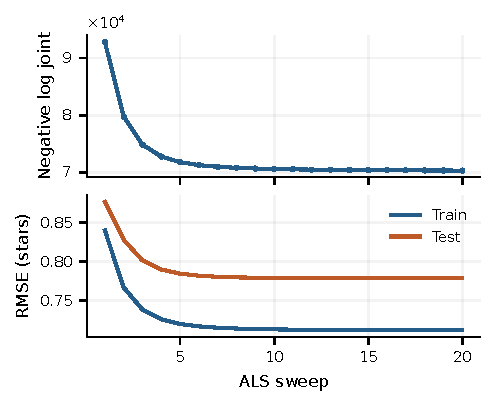
\includegraphics[width=\columnwidth]{practical3_learning_curves.pdf}
\caption{Ten-factor ALS: negative log joint decreases and train/test errors approach a plateau.}
\label{fig:als}\end{figure}

\subsection{Capacity and Regularization}
Twenty factors reduce training RMSE from 0.71 to 0.66, while both test errors round to 0.78. The small unrounded test gain costs 2.22 times more fitting time (Figure~\ref{fig:capacity}; Table~\ref{tab:experiments}).

\begin{figure}[H]
\centering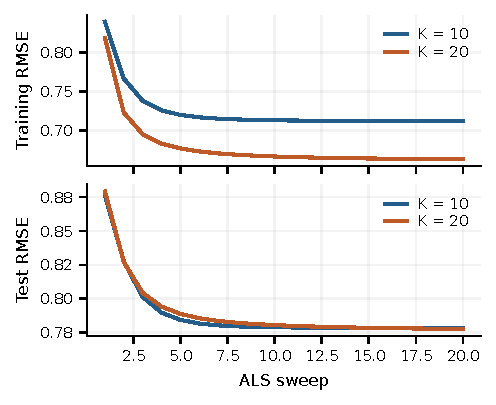
\includegraphics[width=\columnwidth]{capacity_comparison.pdf}
\caption{Training and test RMSE by factor count. Higher capacity lowers training error with little test improvement.}
\label{fig:capacity}\end{figure}
\begin{table}[H]
\caption{ALS comparisons with $\tau_b=0.001$ and 20 sweeps. Train and test columns report RMSE; times include training and evaluation.}
\label{tab:experiments}\centering\small\setlength{\tabcolsep}{2pt}\begin{tabular*}{\linewidth}{@{\extracolsep{\fill}}lrrrrrr}
\toprule
Setting & $K$ & $\lambda$ & $\tau$ & Train & Test & Time (s) \\
\midrule
Baseline & 10 & 0.01 & 0.1 & 0.71 & 0.78 & 190.48 \\
$K=20$ & 20 & 0.01 & 0.1 & 0.66 & 0.78 & 423.75 \\
$\tau=0.01$ & 10 & 0.01 & 0.01 & 0.70 & 0.79 & 198.06 \\
$\tau=1$ & 10 & 0.01 & 1 & 0.77 & 0.80 & 184.43 \\
$\lambda=0.1$ & 10 & 0.1 & 0.1 & 0.70 & 0.79 & 184.50 \\
\bottomrule
\end{tabular*}

\end{table}

Weakening $\tau$ to 0.01 or raising $\lambda$ to 0.1 improves training fit but worsens test RMSE to 0.79. Their test errors reach minima at sweep 12, then rise while the training objective decreases: evidence of overfitting. Raising $\lambda$ also weakens the effective bias penalty. Stronger $\tau=1$ worsens both training and test fit.

Twenty factors help the most-active users but worsen both lower-activity groups (Table~\ref{tab:activity}). The 100+ group contributes most test observations and drives the aggregate gain. Less-active users provide less evidence for larger vectors.

\begin{table}[H]
\caption{Test RMSE by user training activity, using identical observations for both models.}
\label{tab:activity}\centering\small\begin{tabular*}{\linewidth}{@{\extracolsep{\fill}}lrrr}
\toprule
Train ratings & Test rows & $K=10$ & $K=20$ \\
\midrule
1--19 & 101,076 & 0.93 & 0.95 \\
20--99 & 1,365,017 & 0.83 & 0.85 \\
100+ & 4,932,861 & 0.76 & 0.75 \\
\bottomrule
\end{tabular*}

\end{table}

\subsection{Genre Prior and Cold Start}
Genre ALS has training RMSE 0.71 and test RMSE 0.78. Its unrounded test improvement over ten-factor ALS is only 0.10\%; one split does not establish significance. Test error reaches a shallow minimum at sweep 15, but the retained model remains sweep 20 (Figure~\ref{fig:genre}).

\begin{figure}[H]
\centering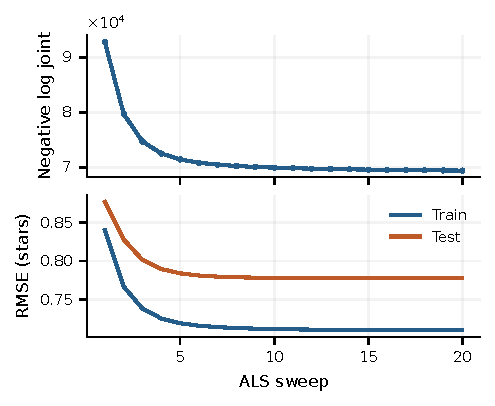
\includegraphics[width=\columnwidth]{genre_learning_curves.pdf}
\caption{Genre ALS: negative log joint decreases; test RMSE has a shallow minimum at sweep 15.}
\label{fig:genre}\end{figure}
\begin{table}[H]
\caption{Warm-user test groups. The controlled study withholds training ratings for 1,063 supported movies.}
\label{tab:cold}\centering\small\begin{tabular*}{\linewidth}{@{\extracolsep{\fill}}lrrr}
\toprule
Test group & Ratings & ALS & Genre ALS \\
\midrule
Warm items & 6,394,233 & 0.78 & 0.78 \\
Natural cold items & 4,721 & 1.03 & 1.04 \\
Controlled cold items & 329,121 & 0.99 & 0.97 \\
\bottomrule
\end{tabular*}

\end{table}

For naturally cold items, genres worsen RMSE from 1.03 to 1.04 (Table~\ref{tab:cold}). This group contains only 4,721 test ratings, so its effect on aggregate error is small.

The controlled study selects 5\% of movies with at least 20 training ratings (seed 43), removes their training observations, and refits both models. Evaluation uses their test ratings from users who retain training data. Independent reconstruction verifies 1,063 movies and 329,121 test observations. Recorded RMSE improves from 0.99 to 0.97 with genres, a 2.22\% reduction calculated before rounding.

Naturally unsupported and deliberately withheld movies are different populations. These results do not show that genres always improve cold start; the controlled study also lacks saved checkpoints for independent error recomputation.

\subsection{Two-Dimensional Fits}
Figures~\ref{fig:movies2d} and~\ref{fig:genres2d} show models trained directly with $K=2$. Nearby Star Wars films and the Crime/Mystery genre pair illustrate learned relationships, but the axes have no intrinsic meaning because joint rotation or reflection preserves dot products. Both test RMSEs round to 0.81, above the main models.

\begin{figure}[H]
\centering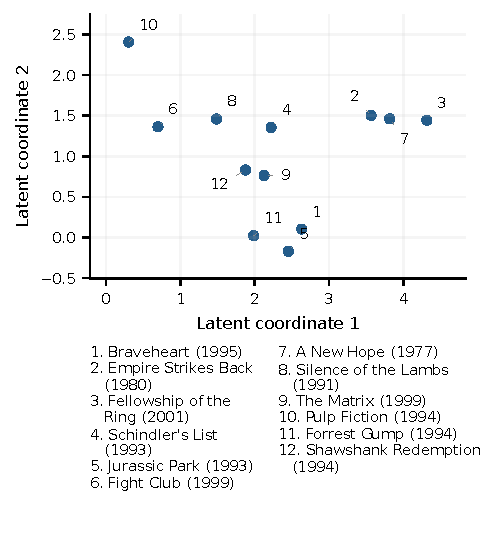
\includegraphics[width=\columnwidth]{movies_2d.pdf}
\caption{Direct two-factor movie fit. Numbers identify twelve frequently rated films; the key uses shortened titles.}
\label{fig:movies2d}\end{figure}
\begin{figure}[H]
\centering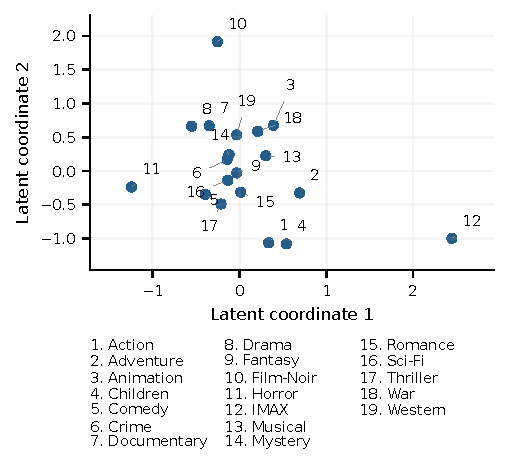
\includegraphics[width=\columnwidth]{genres_2d.pdf}
\caption{Direct two-factor genre fit. Labels are offset without moving the learned coordinates.}
\label{fig:genres2d}\end{figure}
\FloatBarrier
